\documentclass{beamer}
\usepackage[ntu,zh]{collegeBeamer}
\usepackage{booktabs}
\usepackage{amsmath}
\usepackage{array}
\usepackage{multicol}

\renewcommand{\figurename}{图}
\renewcommand{\tablename}{表}
\graphicspath{{assets/}}

\title{RACE：大模型神经元功能一致性的\texorpdfstring{\newline}{}\,可扩展统计估计}
\subtitle{Residual Alignment for Consistency Estimation}
\author{Runyu Wang\inst{1}, Bo Liu\inst{2}, Xiaxin Zhang\inst{1}, Yu Han\inst{1}, Jiawei Cao\inst{1}, \texorpdfstring{\newline}{} Xiaoye Zhang\inst{3}, Zhe Zhang\inst{4}, Yifan Yang\inst{4}, Peng Ping\texorpdfstring{\textsuperscript{*}}{*}\inst{1}}
\institute{\inst{1}南通大学 \quad \inst{2}重庆邮电大学 \quad \inst{3}南方电网 \quad \inst{4}美团 \quad \texorpdfstring{\textsuperscript{*}}{*}通讯作者}
\date{EMNLP 2026 (Award 提名) }

\begin{document}

\maketitle

\section{背景与研究问题}

\begin{frame}{从单样本归因到领域级定位}
    \begin{columns}[T]
        \begin{column}{0.48\textwidth}
            \textbf{现有定位方法的瓶颈}
            \begin{itemize}
                \item \textbf{开销高}：梯度归因与因果干预需反复反向传播或多次运行，难以扩展到大模型与大数据集。
                \item \textbf{信号粗糙}：直接对单样本得分求平均，掩盖了神经元在不同输入间的剧烈波动。
                \item \textbf{附加训练}：稀疏自编码器（SAE）需逐层单独训练字典。
            \end{itemize}
        \end{column}
        \begin{column}{0.48\textwidth}
            \begin{alertblock}{核心目标：定位领域内稳定工作的原生神经元}
                在目标领域（如代码、数学）中，找到\textbf{持续、稳定参与模块更新}的神经元，支撑能力审计、剪枝与行为控制。
            \end{alertblock}
            \vspace{0.2em}
            \textbf{什么是功能一致性？}
            \begin{itemize}
                \item \alert{贡献幅度大}：同向推动当前模块的残差更新。
                \item \alert{跨样本稳定}：在领域内持续生效，而非偶发激活。
            \end{itemize}
        \end{column}
    \end{columns}
\end{frame}

\begin{frame}{RACE 框架概览}
    \begin{columns}[T]
        \begin{column}{0.55\textwidth}
            \centering
            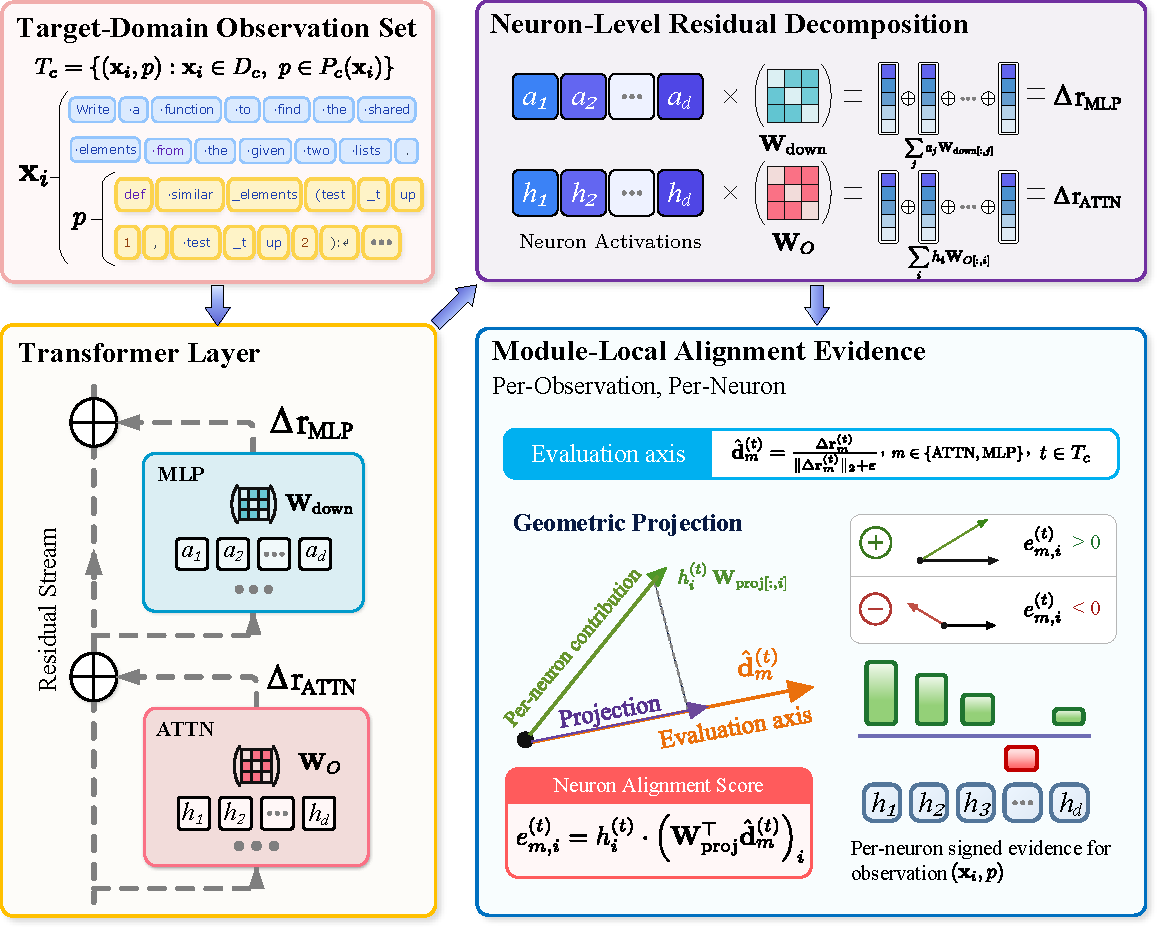
\includegraphics[width=\textwidth,height=0.78\textheight,keepaspectratio]{RACE_pipeline.pdf}
            \vspace{-0.2em}\par
            \centering\scriptsize 图 1：RDA 逐位置提取残差对齐证据
        \end{column}
        \begin{column}{0.41\textwidth}
            \footnotesize
            \begin{enumerate}\setlength{\itemsep}{0.25em}
                \item \textbf{前向取证（RDA）}：将神经元输出投影到所属模块的更新方向，获取有符号对齐证据。
                \item \textbf{贝叶斯聚合（CAM）}：用 NIG 共轭后验融合均值与方差，按置信下界为神经元打分。
                \item \textbf{参考集过滤（RSF）}：剔除在通用语料上同样活跃的神经元，提纯领域特异信号。
            \end{enumerate}
            \vspace{0.3em}
            \begin{block}{零反向传播开销}
                \scriptsize 仅需单次前向传播，流式维护充分统计量（单神经元 $O(1)$ 显存）。
            \end{block}
        \end{column}
    \end{columns}
\end{frame}

\section{方法：前向取证与贝叶斯评分}

\begin{frame}{RDA：模块局部的残差方向对齐}
    \small
    在残差流中，每个模块的输出增量可精确分解为各神经元的秩-1 写入之和（以 MLP 为例）：
    \begin{equation*}
        \Delta r_{\mathrm{MLP}}^{(t)} = W_{\mathrm{down}}a^{(t)}
        = \sum_j a_j^{(t)}W_{\mathrm{down}}[:,j].
    \end{equation*}
    以当前模块的归一化更新方向 $\hat d^{(t)}$ 为参考轴，定义神经元 $j$ 的对齐证据：
    \begin{equation*}
        \hat d^{(t)} = \frac{\Delta r^{(t)}}{\lVert\Delta r^{(t)}\rVert_2+\varepsilon},
        \qquad
        e_j^{(t)} = a_j^{(t)}\,W_{\mathrm{down}}[:,j]^\top\hat d^{(t)}.
    \end{equation*}
    \begin{columns}[T]
        \begin{column}{0.48\textwidth}
            \begin{alertblock}{几何与物理意义}\scriptsize
                $\sum_j e_j^{(t)} = \lVert\Delta r^{(t)}\rVert_2$（精确分解模块更新范数）。\\
                $e_j^{(t)}>0$ 正向推动更新；$e_j^{(t)}<0$ 反向抵消。
            \end{alertblock}
        \end{column}
        \begin{column}{0.48\textwidth}
            \begin{exampleblock}{为什么使用模块局部方向？}\scriptsize
                浅层与中层承担词法、句法或路由功能，尚未对齐最终词表；局部方向可避免后续层的旋转与覆盖干扰。
            \end{exampleblock}
        \end{column}
    \end{columns}
\end{frame}

\begin{frame}{CAM：兼顾贡献幅度与跨样本稳定性}
    将神经元 $j$ 在 $n$ 个观测位置上的证据建模为正态-逆伽马（NIG）共轭模型：
    \begin{equation*}
        e_j^{(t)}\sim\mathcal N(\mu_j,\sigma_j^2),\qquad
        (\mu_j,\sigma_j^2)\sim\mathrm{NIG}(\mu_0,\lambda_0,\alpha_0,\beta_0).
    \end{equation*}
    流式累积均值 $\bar e_j$ 与离差平方和 $\mathrm{SS}_j$，闭式导出均值后验 $t$ 分布的参数：
    \begin{equation*}
        \mu_{n,j}=\frac{\lambda_0\mu_0+n\bar e_j}{\lambda_0+n},
        \qquad
        \sigma_{\mu,j}^2=\frac{\beta_{n,j}}{\alpha_n\lambda_n}.
    \end{equation*}
    \begin{block}{保守对齐幅度（CAM 得分）}
        \begin{equation*}
            \mathrm{CAM}_j(\gamma)=\mathbf 1[\mu_{n,j}>0]
            \max\!\left(0,\mu_{n,j}-t_{1-\gamma,2\alpha_n}\sigma_{\mu,j}\right).
        \end{equation*}
        取均值后验的 $(1-\gamma)$ 单侧置信下界：\textbf{奖励持续正向贡献，自动惩罚偶发激活或正负摇摆的神经元}。
    \end{block}
\end{frame}

\begin{frame}{分层排序与参考集过滤（RSF）}
    \begin{columns}[T]
        \begin{column}{0.52\textwidth}
            \includegraphics[page=6,trim=70 426 300 308,clip,width=0.90\textwidth]{RACE-paper.pdf}
            \vspace{0.05em}\par
            \centering\scriptsize 图 2：CAM 得分随模型加深整体右移
            \vspace{0.25em}\par
            \raggedright\footnotesize
            \textbf{按层独立预算}：深层残差范数与 CAM 数值天然偏大；在每层、每模块内部独立排序选点，保障全模型各层的覆盖度。
        \end{column}
        \begin{column}{0.45\textwidth}
            \footnotesize
            \textbf{参考集过滤（RSF）}：剥离通用语言神经元
            \begin{equation*}
                \Pi_{\mathrm{tar}}^\ell=\mathrm{rank}(\mathrm{CAM}),\quad
                B_{\mathrm{ref}}^\ell=\mathrm{TopK}_{\mathrm{ref}}(D_{\mathrm{ref}}),
            \end{equation*}
            \begin{equation*}
                S_{\mathrm{spec}}^\ell=\mathrm{FirstK}_{\mathrm{sel}}
                \left(\Pi_{\mathrm{tar}}^\ell\setminus B_{\mathrm{ref}}^\ell\right).
            \end{equation*}
            \vspace{-0.3em}
            \begin{block}{过滤流程}
                \scriptsize
                \begin{itemize}
                    \item \textbf{目标集}（MBPP+ / MATH-500）：生成候选排序 $\Pi_{\mathrm{tar}}^\ell$。
                    \item \textbf{参考集}（WikiText-2）：标记通用高分神经元 $B_{\mathrm{ref}}^\ell$。
                    \item \textbf{特异集}：跳过通用神经元，每层选满 $K_{\mathrm{sel}}$ 个目标神经元。
                \end{itemize}
            \end{block}
        \end{column}
    \end{columns}
\end{frame}

\section{实验与分析}

\begin{frame}{实验设置与评估指标}
    \begin{columns}[T]
        \begin{column}{0.45\textwidth}
            \textbf{评测模型（覆盖 4B 至 32B）}
            \begin{itemize}
                \item Qwen3-4B-it（主力评测）
                \item Llama-3.1-8B-it
                \item OLMo-3.1-32B-it（规模验证）
            \end{itemize}
            \vspace{0.4em}
            \textbf{验证方式：定向置零抑制}
            \begin{itemize}
                \item 推理时将选中神经元激活置零
                \item 对比梯度归因（GxAct、AttnLRP）与统计消融基线
            \end{itemize}
        \end{column}
        \begin{column}{0.51\textwidth}
            \scriptsize
            \setlength{\tabcolsep}{4pt}
            \begin{tabular}{>{\bfseries}l l l}
                \toprule
                任务领域 & 评分集 $D_{\mathrm{tar}}$ & 同域泛化 (OOD) \\
                \midrule
                代码生成 & MBPP+ & HumanEval+ \\
                数学推理 & MATH-500 & AMC \\
                细粒度语法 & PyComp-1K & MBPP+ / HumanEval+ \\
                \bottomrule
            \end{tabular}
            \vspace{0.2em}\par
            {\scriptsize 通用保留基准：MMLU-Redux、GPQA、ARC；参考集：WikiText-2。}
            
            \vspace{0.2em}
            \begin{alertblock}{干预特异性指数（ISI $\uparrow$）}
                \scriptsize
                $$\mathrm{ISI} = \max\left\{0, \log\left(\frac{\Delta_T}{\Delta_G + \delta}\right)\right\}$$
                衡量\textbf{目标领域相对跌幅 $\Delta_T$} 与\textbf{非目标领域跌幅 $\Delta_G$} 的对数比值。ISI 越高，说明干预越精准。
            \end{alertblock}
        \end{column}
    \end{columns}
\end{frame}

\begin{frame}{领域特异性干预：精准抑制目标能力}
    \begin{columns}[T]
        \begin{column}{0.58\textwidth}
            \includegraphics[page=7,trim=40 625 40 55,clip,width=\textwidth]{RACE-paper.pdf}
            \vspace{-0.4em}\par
            \centering\scriptsize 图 3：Qwen3-4B-it 上抑制各层 Top-1\% 神经元后的准确率保留比例与 ISI
        \end{column}
        \begin{column}{0.40\textwidth}\scriptsize
            \begin{block}{Qwen3-4B-it（Top-1\% MLP 抑制）}
                \begin{itemize}
                    \item \textbf{代码域}：MBPP+ ($82.3\%\to 3.2\%$)，同域 HumanEval+ ($83.5\%\to 1.2\%$)；MMLU 保持 $82.4\%$，\alert{\textbf{ISI = 2.65}}。
                    \item \textbf{数学域}：MATH-500 ($94.4\%\to 29.0\%$)，同域 AMC ($87.3\%\to 11.9\%$)；\alert{\textbf{ISI = 1.76}}。
                \end{itemize}
            \end{block}
            \vspace{-0.2em}
            \begin{block}{跨模型扩展（OLMo-32B 数学域 MLP）}
                \begin{itemize}
                    \item 抑制 Top-1\%：MATH-500 从 $86.4\%$ 降至 $56.8\%$，AMC 从 $79.9\%$ 降至 $14.2\%$，MMLU 保持 $82.7\%$（\textbf{ISI = 1.65}）。
                \end{itemize}
            \end{block}
        \end{column}
    \end{columns}
\end{frame}

\begin{frame}{分布偏移与细粒度行为控制}
    \begin{columns}[T]
        \begin{column}{0.47\textwidth}
            \footnotesize
            \textbf{1. 预测分布的非对称破坏（MLP Top-1\%）}
            \vspace{0.1em}
            \begin{center}
            \scriptsize
            \setlength{\tabcolsep}{4pt}
            \begin{tabular}{l|ccc}
                \toprule
                干预设置 & MBPP+ & MATH-500 & WikiText-2 \\
                \midrule
                代码域 ($\Delta\text{PPL}$) & \alert{\textbf{+77.3\%}} & +24.0\% & \textbf{+2.8\%} \\
                数学域 ($\Delta\text{PPL}$) & +25.4\% & \alert{\textbf{+129.0\%}} & \textbf{+2.6\%} \\
                \bottomrule
            \end{tabular}
            \end{center}
            \vspace{-0.2em}
            \begin{itemize}\scriptsize
                \item 目标域困惑度大幅飙升，而通用语料 WikiText-2 几乎不受影响（$<3\%$），底层语言能力完好。
            \end{itemize}

            \vspace{0.1em}
            \textbf{2. 为什么 MLP 比 ATTN 更具领域特异性？}
            \begin{itemize}\scriptsize
                \item 三域 Top-1\% 神经元 Jaccard 重叠率：\textbf{ATTN 为 0.264，MLP 仅为 0.085}（相差 $3.1\times$）。
                \item ATTN 跨领域复用度高，承担通用路由；MLP 神经元分工更专一。
            \end{itemize}
        \end{column}
        \begin{column}{0.49\textwidth}
            \footnotesize
            \textbf{3. 细粒度语法引导：抑制 Python 推导式}
            \begin{itemize}\scriptsize
                \item 用 1,000 条含推导式的语句（PyComp-1K）定位并抑制每层 10 个神经元：
            \end{itemize}
            \begin{center}
            \scriptsize
            \setlength{\tabcolsep}{3.5pt}
            \begin{tabular}{l|cc|cc}
                \toprule
                & \multicolumn{2}{c|}{\textbf{MBPP+}} & \multicolumn{2}{c}{\textbf{HumanEval+}} \\
                策略 & 推导式 & 通过率 & 推导式 & 通过率 \\
                \midrule
                原始模型 & 55 & 92.7\% & 36 & 86.1\% \\
                RACE & \alert{\textbf{16 (-70.9\%)}} & \textbf{87.5\%} & \alert{\textbf{14 (-61.1\%)}} & \textbf{85.7\%} \\
                \bottomrule
            \end{tabular}
            \end{center}
            \begin{alertblock}{精准改变代码风格而非破坏逻辑}\scriptsize
                模型大幅减少列表/字典推导式的使用，转而生成等价的循环结构，代码功能通过率保持稳定。
            \end{alertblock}
        \end{column}
    \end{columns}
\end{frame}

\begin{frame}{计算开销与核心组件消融}
    \begin{columns}[T]
        \begin{column}{0.46\textwidth}
            \footnotesize
            \textbf{计算开销对比（Qwen3-4B-it）}
            \begin{center}
            \scriptsize
            \setlength{\tabcolsep}{4pt}
            \begin{tabular}{lrr}
                \toprule
                方法 & 额外计算量 & 相对前向开销 \\
                \midrule
                GxAct & 18.77 TFLOPs & 144.29$\times$ \\
                AttnLRP & 18.82 TFLOPs & 144.62$\times$ \\
                \textbf{RDA (RACE)} & \textbf{81.5 GFLOPs} & \alert{\textbf{0.63$\times$}} \\
                \bottomrule
            \end{tabular}
            \end{center}
            \vspace{-0.3em}
            \begin{itemize}\scriptsize
                \item \textbf{百倍加速}：评分开销不到梯度方法的 \textbf{1/200}。
                \item \textbf{极低显存}：仅需 \textbf{0.95 MB} 状态存储，峰值显存与常规推理一致。
            \end{itemize}
            \centering
            \includegraphics[page=9,trim=55 680 302 75,clip,width=0.68\textwidth]{RACE-paper.pdf}
            \vspace{0.05em}\par
            \scriptsize 图 4：不同样本量 $N$ 下 RACE 始终优于经验均值
        \end{column}
        \begin{column}{0.50\textwidth}
            \footnotesize
            \textbf{评分准则消融（代码域 MLP，$K_{\mathrm{sel}}=5$）}
            \begin{center}
            \scriptsize
            \setlength{\tabcolsep}{3.5pt}
            \begin{tabular}{l|cc|c}
                \toprule
                评分方法 & HumanEval+ $\downarrow$ & MMLU $\uparrow$ & \textbf{ISI} $\uparrow$ \\
                \midrule
                原始模型 & 83.54 & 81.37 & — \\
                \midrule
                GxAct (梯度) & 5.49 & 15.25 & 0.04 \\
                Act. Mean (仅激活) & 3.66 & 81.18 & 2.22 \\
                Emp. SNR (信噪比) & 86.59 & 81.23 & 0.00 \\
                Emp. Mean (经验均值) & 0.00 & 81.33 & 2.79 \\
                \textbf{RACE (CAM)} & \alert{\textbf{0.00}} & \textbf{81.79} & \alert{\textbf{2.91}} \\
                \bottomrule
            \end{tabular}
            \end{center}
            \vspace{-0.5em}
            \begin{alertblock}{为什么需要贝叶斯方差正则化？}\scriptsize
                \begin{itemize}
                    \item \textbf{Emp. SNR 失效（ISI=0）}：稀疏激活下样本方差趋近于 0，微弱噪点被放大。
                    \item \textbf{CAM 稳健性}：NIG 先验提供非零方差下界，过滤稀疏噪声，始终保持最高选择性。
                \end{itemize}
            \end{alertblock}
        \end{column}
    \end{columns}
\end{frame}

\section{总结}

\begin{frame}{总结}
    \begin{block}{核心工作}
        \begin{enumerate}\setlength{\itemsep}{0.4em}
            \item \textbf{前向残差对齐（RDA）}：在模块局部更新方向上精确分解神经元写入，以 $0.63\times$ 前向开销替代高昂的梯度反传。
            \item \textbf{保守对齐幅度（CAM）}：基于 NIG 共轭后验的置信下界打分，同时锁定高贡献与跨样本高稳定性的神经元。
            \item \textbf{分层参考集过滤（RSF）}：消除网络深度偏置并剥离通用语言神经元，揭示了 MLP 相比 ATTN 具有更强的领域专一性（跨领域重叠低 $3.1\times$）。
            \item \textbf{精准干预能力}：在 4B--32B 模型上实现代码、数学及特定语法风格（Python 推导式）的定向抑制，保持非目标通用能力不受损。
        \end{enumerate}
    \end{block}
    \vfill
    \centering\small\bhref{https://github.com/Nexround/RACE}{开源代码与数据：github.com/Nexround/RACE}
\end{frame}

\QApage

\end{document}
